\documentclass[a4paper]{article}

\usepackage[usenames,dvipsnames]{color}
\usepackage[utf8]{inputenc}
\usepackage{graphicx}

\title{Ethon - Design}
\author{David}
\begin{document}
\maketitle 

\section{Introducción}

¿Desarrollar un motor propio o usar uno que ya exista?. Cada vez que me he planteado desarrollar un viedeojuego me he hecho la misma pregunta y la mayoría de las veces siempre he acabando desarrollando un pequeño motor basado en otro o desde cero para satisfacer mis necesidades.

Hace poco me he vuelto a hacer la misma pregunta para un proyecto de la universidad de desarrollar un juego en HTML5 y decidí hacer un poco de reflexión personal. He pensado en cuatro puntos que me hacen decantar por el desarrollo de un motor propio:

\begin{itemize}
  \item \textbf{Motivación personal:} Hace ya algunos años que intento dedicarme a esto, pero de momento solo he conseguido hacer cosas a modo de hobby. Durante los pequeños desarrollos que he hecho siempre me he construido ``pequeños motores'' sin sentido alguno. Es una espina que tengo clavada desde hace tiempo y creo que en este proyecto puedo conseguir hacer alguna cosa más seria.
  \item \textbf{Ingeniería:} Aunque a veces me arrepiento, vengo de la Ingeniería informática. Durante 5 años nos enseñaron la teoría de como debía ser un buen software, su diseño, etc. Implementar un motor de videojuegos es una tarea difícil, que requiere mucho esfuerzo e ingenería para poder ensamblar todos los módulos del juego. Aunque también me gusta programar el gameplay del juego, diseñar un motor siempre ha sido una de mis metas.

  \item \textbf{Tiempo:} Aunque parezca contradictorio también es un motivo, me explico. Durante el dia me quedan pocas horas para dedicar a la universidad a causa del trabajo, el perro y el piso. En el trabajo estamos explorando el tema del gaming en HTML5 y estamos desarrollando un producto propio que va a necesitar de este motor. En resumen, puedo dedicar algunas horas del trabajo a implementar parte del motor.

  \item \textbf{Diversión:} Diseñar e implementar un motor de videojuegos es divertido. Te permite experimentar con todos los ámbitos del videojuego y profundizar en algunos de ellos. Debo reconocer que parte de mi sigue pensando en el desarrollo de videojuegos como hobby aunque cada día que pasa creo más en poder dedicarme a esto profesionalmente en un futuro.
\end{itemize}

Tras esta reflexión puedo empezar a desarrollar un motor definiendo los requisitos mínimos que ha de tener para poder empezar a usarlo.

\section{Requisitos}

Ya que voy a definir los requisitos de un motor para crear videojuegos creo que una buena forma de hacerlo es a través de ejemplos reales. Usaré dos videojuegos bien conocidos: \textbf{pong} y \textbf{pac-man} para averiguar que necesito para crear un motor usable en HTML5.

\subsection{Pong}

Pong fue un videojuego de la primera generación de videoconsolas publicado por Atari, creado por Nolan Bushnell y lanzado el 29 de noviembre de 1972. Está basado en el deporte de tenis de mesa o \textit{ping pong}.

\begin{figure}[h]
  \begin{center}
    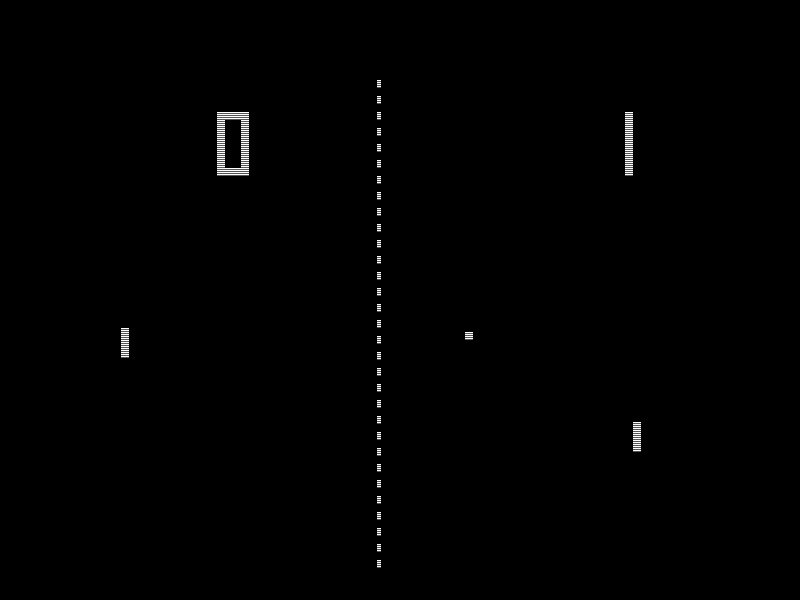
\includegraphics[width=250px]{images/pong.png}
    \caption{Captura de pantalla del videojuego Pong}
    \label{pong}
  \end{center}
\end{figure}

Para el diseño del motor he pensado en hacer alguna variación sencilla del juego pero sin perder la esencia de este. El objetivo del juego es \textbf{llegar a 7 puntos} y conseguiremos un punto \textbf{cada vez que la pelota atraviese el campo del rival}. \\
Acabamos de definir la \textbf{condición de victoria} del juego y a su vez también la \textbf{condición de derrota}. Entonces podemos dividir el juego en tres estados:
\begin{itemize}
  \item \textbf{Juego:} El estado normal del juego.
  \item \textbf{Victoria:} Cuando llegamos a 7 puntos aparece un mensaje diciendo que hemos ganado.
  \item \textbf{Derrota:} Si el rival llega a 7 puntos aparece un mensaje diciendo que hemos perdido.
\end{itemize}

Nuestro motor debe permitir definir estos \textbf{estados de juego} así como las \textbf{transiciones} entre ellos. Una vez hemos visto que necesitamos crear hasta 3 estados de nuestro juego, empezaremos a trabajar en cada uno de ellos y analizaremos lo que el motor debe proporcionarnos para poder implementarlos.


Podemos ver el estado principal del pong en la figura \ref{pong}. En la imagen podemos apreciar los siguientes elementos:

\begin{itemize}
  \item \textbf{Elementos estáticos:} El fondo, la red y las puntuaciones.
  \item \textbf{Elementos dinámicos:} Las palas y la pelota.
\end{itemize}

\subsubsection{Elementos estáticos}

Empezaremos por el grupo de \textbf{elementos estáticos}. Si los analizamos uno por uno, podemos ver como el fondo es un elemento que se debe dibujar antes que los demás, ocupará toda la pantalla y no requiere de ninguna actualización. Acabamos de introducir las palabras claves de \textbf{dibujar} y \textbf{actualizar} que corresponden al ciclo básico del motor de videojuegos.
El fondo del juego será un \textbf{rectangulo de color negro} que ocupará toda la pantalla. 

Nuestro motor debe ser capaz de \textbf{dibujar rectangulos de cualquier tamaño y color}. Aún siendo un elemento estático, este tendrá una \textbf{posición} y un \textbf{tamaño}. Parece lógico crear una entidad reusable en el motor que se encargue de mantener estos valores. En el contexto del motor llamaremos a estas entidades \textbf{souls}.

Tenemos dos \textbf{souls} más en nuestros elementos estáticos: la red y las puntuaciones. En el caso de la red, la representaremos con una serie de cuadrados discontinuos. Como podemos ver, cada \textbf{alma} tiene su propio método de dibujo. Deberemos extraer la lógica de pintado común de los elementos mencionados anteriormente en una entidad común. La llamaremos \textbf{render assistant} y lo usaremos para dibujar en las funciones de dibujo de los elementos.

Para acabar con la lista de elementos estáticos, tenemos las puntuaciones. En este caso cada puntuación se representa con un número que indica la puntuación del jugador correspondiente. Nuestro \textbf{render assistant} deberá ser capaz de \textbf{dibujar texto de diferente tamaño y color}. Al contrario de los elementos estáticos anteriores, éste deberá ser actualizado acorde a la puntuación de cada jugador. No será responsabilidad de la puntuación comprobar si el jugador ha puntuado o no sinó que \textbf{estará a la espera de recibir órdenes}. Con esta última frase acabamos de introducir otro elemento clave del motor y es el \textbf{sistema de publicación y subscripción de eventos}. Introduciremos de nuevo este concepto cuando hablemos de los elementos dinámicos.

\subsubsection{Elementos dinámicos}

Los elementos dinámicos son aquellos que no se mantienen en una posición fija y que se mueven durante el transcurso del juego. A efectos del motor, serán \textbf{souls} que tendrán \textbf{velocidad} en momentos determinados.

Primero hablaremos de las palas. En el juego habrá dos: la pala de la izquierda que representa al jugador, es decir, \textbf{la persona que interactúa con el ordenador y juega al juego} y la pala de la derecha que representa al rival, en nuestro caso una pala manipulada por la \textbf{IA} del juego.

En el párrafo anterior hemos introducido dos nuevos conceptos en nuestro motor: la \textbf{interacción del usuario con el juego} y la \textbf{inteligencia artificial}. Para el caso de la interacción, nos centraremos en el uso del \textbf{teclado} y el \textbf{ratón}. El motor necesitará un \textbf{input assistant} que se encargue de registrar la entrada del jugador para su consulta posterior por parte del juego. \\
Para la inteligencia artificial podemos empezar por algo muy básico, como una máquina de estados sencilla. En el caso del pong, el rival será una pala que seguirá la pelota para poder devolverla. Es un comportamiento muy básico y en este caso no requiere de ninguna implementación adicional. No obstante, hablaremos de que nos puede aportar el motor para este campo en concreto más adelante.

Volviendo al \textbf{input assistant} del motor, hemos dicho que éste módulo será capaz de leer el estado del teclado y el estado del ratón para su posterior uso. El juego necesitará saber el estado de estos elementos para decidir \textbf{acciones} que se llevaran a cabo por parte del jugador. Por ejemplo, si movemos el ratón la pala deberá seguirlo o si presionamos la tecla flecha inferior la pala se moverá hacia abajo. Para éste juego en concreto he preferido usar el ratón como mecanismo para mover el jugador. Queremos separar al máximo los \textbf{dispositivos de entrada} de las \textbf{acciones del jugador}. Para ello nuestro motor nos proporcionará un \textbf{action dispatcher} que actuará entre mediador de los dispositivos de entrada y el juego. Este nuevo módulo usará un mecanismo de \textbf{publicación y subscripción de eventos} del qual hemos hablado con anterioridad.

Habrá algunos componentes del motor y también del juego que implementaremos que serán capaces de \textbf{generar eventos} que otros componentes deberán poder \textbf{escuchar y actuar en consecuencia}. Para poder implementar este mecanismo en nuestro motor necesitaremos un \textbf{event moderator} que se encargue de recibir los eventos y avisar a otros componentes de que ese evento se ha producido y también vamos a proporcionar un componente reusable llamado \textbf{event emitter} que dote a nuestros componentes del mecanismo de subscripción y publicación de eventos.

Hemos definido algunos componentes más del motor pero estabamos hablando de las palas del pong. Recapitulando un poco, podemos definir estos elementos estáticos en un lenguaje que nuestro motor pueda entender. Las palas seran \textbf{almas} que se dibujarán con un rectangulo blanco. La pala del jugador responderá a acciones del jugador mediante la suscripción al \textbf{action dispatcher} que a su vez consultará el estado del ratón mediante el \textbf{input assistant}. La pala del rival se moverá siguiendo la posición de la pelota. A continuación presentaremos el último elemento dinámico del juego pong y acabaremos de definir los requisitos finales del motor.

La pelota es el último dinámico del juego que vamos a describir pero también es el más importante, pues sin ella no se podría jugar. Ambos jugadores deben conseguir que la pelota supere al rival y así puntuar. Dicha pelota en nuestro motor se considerará como un \textbf{alma} con una velocidad constante. La velocidad de la pelota variará en golpear a una de las palas, es decir, rebotará. Todavía no hemos hablado de \textbf{colisiones} y ahora es un buen momento. Recordemos que en nuestro motor solo existe el concepto de \textbf{alma}, entidades con una posición, velocidad y rutinas de dibujo y actualización. Para poder trabajar con colisiones necesitaremos que estas \textbf{almas} tengan un cuerpo. El cuerpo normalmente guardará relación con la imágen del alma, es decir, la pelota tendrá un cuerpo circular y las palas un cuerpo rectangular. Dichos cuerpos tendrán unas \textbf{dimensiones} y una \textbf{forma}, información que usará un nuevo componente del motor llamado \textbf{physics assistant} que se encargará de registrar y avisar de todas las colisiones entre cuerpos. Estos avisos también usaran nuestro sistema de eventos. Entonces la pelota podrá subscribirse al evento de choque con pala para poder reaccionar en consecuencia.

Hemos analizado el estado principal del juego del pong y hemos definido prácticamente los requisitos mínimos de nuestro motor. Nos quedan dos estados más del juego pong pero tras la explicación anterior quedan como estados triviales, donde solo tendremos que mostrar un texto en pantalla y permitir al jugador volver a empezar la partida mediante la pulsación de alguna tecñla, nada nuevo que no hayamos comentado con anterioridad.

\subsection{Pac-man}

Tras analizar el juego del pong y ver los requisitos que necesitamos para el motor pasamos a analizar un juego completamente diferente, el \textbf{pac-man}.

El \textbf{pac-man} es un videojuego arcade creado por el diseñador de videojuegos Toru Iwatani de la empresa Namco. El juego fué lanzado el 21 de mayo de 1980 y fue un gran éxito.  He escogido este juego como el segundo ejemplo para desarrollar el motor ya que requiere algunas características no mencionadas por ahora.

A diferencia del \textbf{pong} éste juego se divide en varias fases donde el objetivo del jugador es \textbf{comer todos los ``cocos'' de la pantalla sin ser comido por los fantasmas}. En cada fase la dificultad puede aumentar de diferentes formas y nuevamente vamos a hacer alguna variación del juego original. Intentaremos crear hasta tres frases con un escenario y ``cocos'' distintos en cada una de ellas.

\begin{figure}[h]
  \begin{center}
    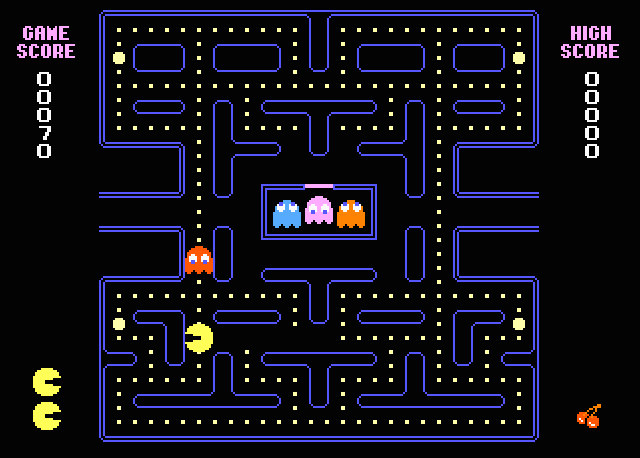
\includegraphics[width=250px]{images/pacman.png}
    \caption{Captura de pantalla del videojuego Pacman}
    \label{pacman}
  \end{center}
\end{figure}

Analizaremos directamente el estado principal del juego ya que los demás estados son muy parecidos al pong y ya hemos hablado anteriormente de los \textbf{estados de juego}. En la figura \ref{pacman} podemos ver una captura de pantalla del juego. Empezaremos el análisis de la misma forma, haciendo un listado de los elementos que podemos ver en pantalla y clasificandolos en estáticos y dinámicos de nuevo:

\begin{itemize}
  \item \textbf{Elementos estáticos:} Fondo, Paredes, Cocos, Cocos especiales, Puntuación actual, Máxima puntuación, Vidas.
  \item \textbf{Elementos dinámicos:} Pacman y los fantasmas.
\end{itemize}

A continuación analizaremos cada uno de los elementos para ir descubriendo nuevas funcionalidades del motor.

\subsubsection{Elementos estáticos}

El fondo del juego vuelve a ser un rectangulo de color negro, nada nuevo por aquí. A continuación nos fijamos en las paredes: elementos estáticos que impiden el paso del jugador y de los enemigos. Hay dos tipos de paredes: las paredes internas de la fase y las paredes externas. La unica variación entre ellas es la \textbf{imagen} que las representa. Podremos usar nuestras \textbf{souls} definidas anteriormente pero ésta vez deberemos ser capaces de \textbf{dibujar una imagen} en lugar de una primitiva básica. Además estás paredes deberan disponer de un \textbf{cuerpo} para poder colisionar con el personaje y los enemigos.

Hagamos un paréntesis y analizemos la imagen del juego (ver figura \ref{pacman}). Podemos imaginar una cuadrícula en la fase que divide cada una de sus partes en \textbf{tiles}, donde cada tile puede ser una pared o vacío. Para simplificarlo, podríamos pensar en unos y ceros. En nuestro caso, un uno puede significar una pared que el jugador no podrá atravesar y un cero puede reprsentar un espacio vacío que el jugador podrá atravesar. \\
Esta división es común en muchos videojuegos en 2D y los motores que se basan en esta tecnología se les llama \textbf{Tile-based engines}. Nuestro motor necesitará implementar algun sistema de \textbf{tiles} para poder representar este escenario. Para ello dispondremos de un módulo llamado \textbf{tile map} que nos permitirá representar este tipo de videojuegos. En nuestro caso tendremos valores superiores a 1 para las paredes y 0 representará un espacio vacío.

Dibujaremos el mapa antes que nuestras \textbf{souls}, ¿pero podríamos considerar el mapa como un \textbf{soul} más?. Yo pienso que no, que se deben considerar entidades separadas. También hemos analizado algunos elementos como las puntuaciones que tampoco son exactamente \textbf{souls}. Nuestro motor dibujará el juego en tres partes: \textbf{el mapa}, \textbf{las souls} y \textbf{la GUI}. Éste último agrupará aquellos elementos que quedarán por encima de los demás. Hemos comentado muy brevemente \textbf{la GUI} cuando hemos hablado de dibujar el texto de las puntuaciones en el juego del pong. La GUI suele estar formado por muchos otros elementos tales como botones, ventanas, etc. Queremos mantener el motor en el mínimo de funcionalides posibles priorizando por ahora solo las \textbf{etiquetas}. Llamaremos \textbf{etiqueta} a cualquier elemento de texto que pertenezca a la interfaz de usuario.

Cerremos el paréntesis y continuemos con el análisis, siendo el turno de los ``cocos''. Estas \textbf{almas} se dibujaran mediante un círculo y estarán repartidas en las casillas vacías del escenario. Cuando el jugador entre en contacto con ellos desapareceran y cuando hayan desaparecido todos el jugador pasará a la siguiente fase. Los ``cocos'' especiales, tal y como indica el nombre, serán clave en el juego. A parte de tener un tamaño mayor al habitual, durante unos segundos proporcionarán al jugador inmunidad a los enemigos y además éstos serán vulnerables al jugador. Si el jugador entra en contacto con un enemigo durante éste estado, el enemigo volverá a su posición inicial. Volveremos a hablar de éste tema en la sección de elementos dinámicos. Nada nuevo para el motor, lógica del juego por ahora.

Para acabar con los elementos estáticos, tan solo nos faltarán las puntuaciones que como ya hemos dicho serán \textbf{etiquetas} de la GUI y el indicador de vidas. En el juego original éste indicador se representaba mediante imágenes de pacman pero como queremos simplificar la interfaz del usuario lo dejaremos como una \textbf{etiqueta} adicional.

\subsubsection{Elementos dinámicos}

\section{MVP - \textit{Minimum Viable Product}}

En esta sección recogeremos todas las funcionalidades necesarias para poder empezar a usar el motor para nuestros juegos. 

\begin{itemize}
  \item Game states
  \item Render assistant
  \begin{itemize}
    \item Draw quads
    \item Draw circles
    \item Draw text
    \item Draw images
  \end{itemize}
  \item Input assistant
  \begin{itemize}
    \item Read keyboard status
    \item Read mouse status
  \end{itemize}
  \item Action dispatcher
  \item Events
  \begin{itemize}
    \item Event moderator
    \item Event emitter
  \end{itemize}
  \item Soul
  \begin{itemize}
    \item Position
    \item Velocity
    \item Render
    \item Update
    \item Body
    \begin{itemize}
      \item Dimensions
      \item Shape
    \end{itemize}
  \end{itemize}
  \item Map
  \begin{itemize}
    \item Tile map
  \end{itemize}
  \item GUI
  \begin{itemize}
    \item Labels
  \end{itemize}
  \item Physics assistant
\end{itemize}

\section{Arquitectura}

\end{document}
